\section{Layout}

Com todos os blocos definidos e o esquemático elétrico desenvolvido, foi possível iniciar o desenvolvimento do layout. Todo o projeto foi realizado utilizando a ferramenta \textit{Virtuoso}, da \textit{Cadence}, utilizando o processo \textit{TSMC CMOS 180 nm}.

A \autoref{layoutcompleto} apresenta a implementação completa do Receptor Óptico projetado. A \autoref{layoutcompleto_division} mostra a mesma figura explicitando o que representa as diferentes partes do circuito. O projeto do Receptor Óptico ocupa uma área total de 633,9x666,96 $\mu$m\textsuperscript{2} ($\approx$~0,423 mm\textsuperscript{2}).

Alguns dos blocos auxiliares do receptor foram desenvolvidos por \textit{Felipe Magalhães} (autor deste trabalho) e \textit{Daniel Carvalho Lott} em seus projetos de Iniciação Cientifica. Os layouts desses blocos estão apresentados de maneira implícita junto aos circuitos apresentados ao longo de todo capítulo.

\begin{figure}[!h]
 \centering
    \caption{Layout completo do circuito desenvolvido} 
    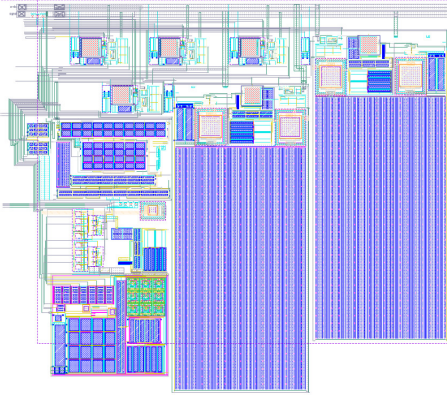
\includegraphics[scale=1, angle = 90]{Projeto/Layout/Imagens/Circuito Completo.png}
    \legend{Fonte: Produzido pelo autor}
    \label{layoutcompleto}
    \nota{Imagem rotacionada em 90° em sentido anti-horário}
\end{figure}

\begin{figure}[!h]
 \centering
    \caption{Layout completo do circuito particionado} 
    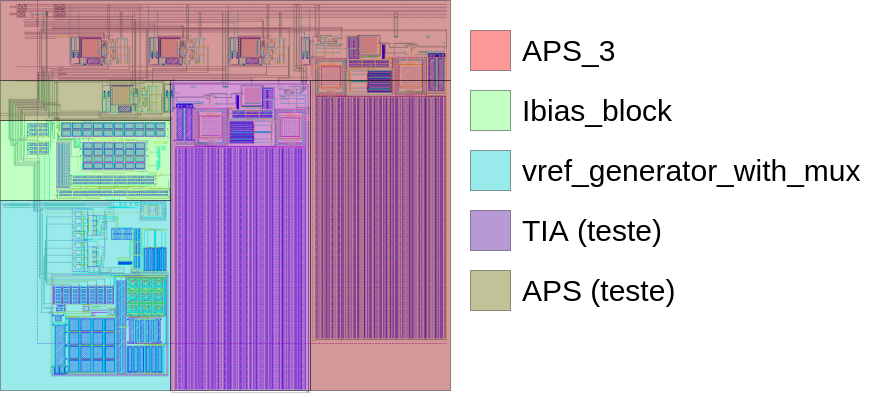
\includegraphics[scale=0.4]{Projeto/Layout/Imagens/Image_CircuitoCompleto.png}
    \legend{Fonte: Produzido pelo autor}
    \label{layoutcompleto_division}
\end{figure}

O bloco \textit{APS\_digitalized} projetado é apresentado na figura \autoref{layoutAPSDIG}. A \autoref{layoutAPSDIG_division} mostra a mesma figura explicitando o que representa as diferentes parte do circuito. O projeto do bloco ocupa uma área total aproximada de 3307 $\mu$m\textsuperscript{2}.

\begin{figure}[!h]
 \centering
    \centering
    \caption{Layout do bloco \textit{APS\_digitalized}} 
    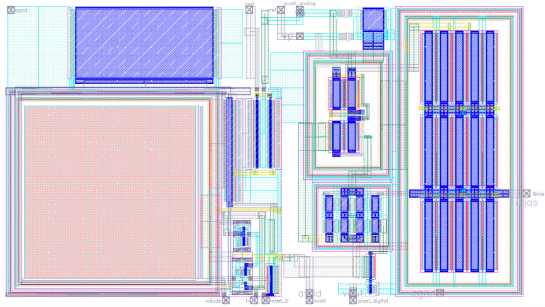
\includegraphics[scale=0.8]{Projeto/Layout/Imagens/APS_DIGITALIZED.png}
    \legend{Fonte: Produzido pelo autor}
    \label{layoutAPSDIG}
\end{figure}

\begin{figure}[!h]
 \centering
    \centering
    \caption{Layout do bloco \textit{APS\_digitalized} particionado} 
    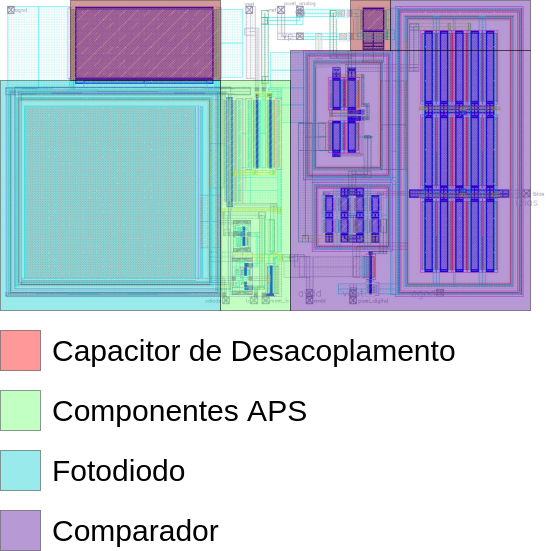
\includegraphics[scale=0.3]{Projeto/Layout/Imagens/Image_APS_Digitalized.png}
    \legend{Fonte: Produzido pelo autor}
    \label{layoutAPSDIG_division}
\end{figure}

O bloco \textit{APS\_clk} projetado é apresentado na figura \autoref{layoutTIA}. A \autoref{layoutTIA_division} mostra a mesma figura explicitando o que representa as diferentes parte do circuito. O projeto do bloco ocupa uma área total aproximada de 102107 um\textsuperscript{2}.

\begin{figure}[!h]
 \centering
    \begin{minipage}{0.5\textwidth}
    \centering
    \caption{Layout do bloco \textit{APS\_clk}} 
    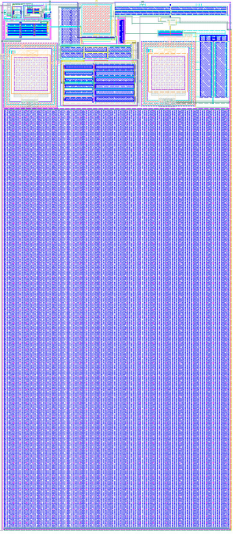
\includegraphics[scale=0.7]{Projeto/Layout/Imagens/TIA.png}
    \legend{Fonte: Produzido pelo autor}
    \label{layoutTIA}
    \end{minipage}
    \hfill
    \begin{minipage}{0.4\textwidth}
    \centering
    \caption{Layout do bloco \textit{APS\_clk} particionado}
    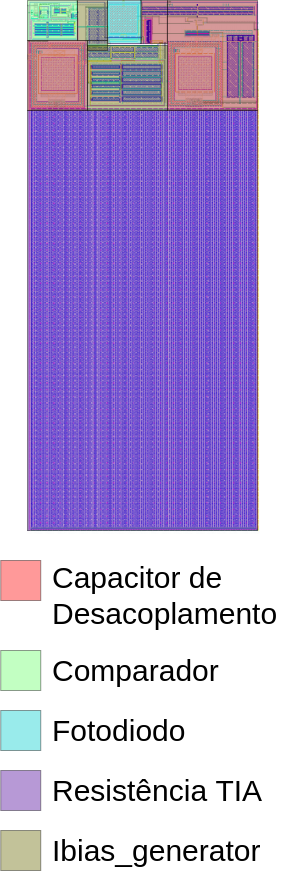
\includegraphics[scale=0.4]{Projeto/Layout/Imagens/Image_TIA.png}
    \legend{Fonte: Produzido pelo autor}
    \label{layoutTIA_division}
    \end{minipage}
\end{figure}

O bloco \textit{APS\_3} projetado é apresentado na figura \autoref{layoutAPS_3}. A \autoref{layoutAPS_3_division} mostra a mesma figura explicitando o que representa as diferentes parte do circuito. O projeto do bloco ocupa uma área aproximada de 123353 $\mu$m\textsuperscript{2}.

\begin{figure}[!h]
    \centering
    \caption{Layout do bloco \textit{APS\_3}} 
    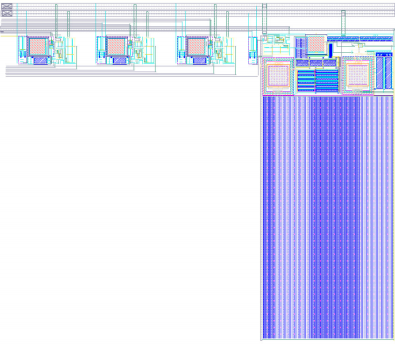
\includegraphics[scale=1]{Projeto/Layout/Imagens/APS_3.png}
    \legend{Fonte: Produzido pelo autor}
    \label{layoutAPS_3}
\end{figure}

\begin{figure}[!h]
    \centering
    \caption{Layout do bloco \textit{APS\_3} particionado} 
    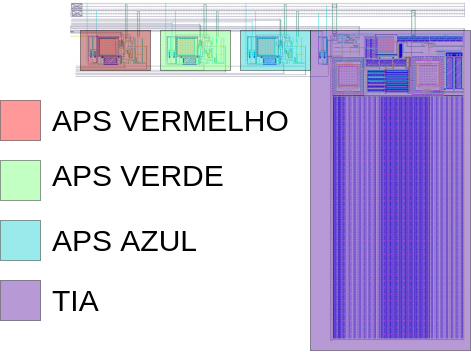
\includegraphics[scale=0.4]{Projeto/Layout/Imagens/Image_APS_3.png}
    \legend{Fonte: Produzido pelo autor}
    \label{layoutAPS_3_division}
\end{figure}

\clearpage

\section{Chip}

O circuito integrado apresentado na \autoref{fig_circintegrado} foi desenvolvido, contendo todo o projeto de Receptor Óptico além de outros projetos desenvolvidos por terceiros. A \autoref{fig_circintegrado_division} mostra de maneira explicita o que representa cada parte do CI, e referências aos outros projetos desenvolvidos.

O circuito integrado apresenta uma área total de 1,6x1,6 mm\textsuperscript{2} (2,56 mm\textsuperscript{2}), utilizando um encapsulamento do tipo CLCC44\footnote{Especificações do encapsulamento presentes no \autoref{anexo_clcc44}}. A \autoref{tab_clcc44} apresenta a relação da numeração dos pinos do encapsulamento com os pinos chip, que são distintos, além da identificação de cada pino.

Diversos capacitores de desacoplamento foram incluídos ao longo de todo chip, com o objetivo de preencher áreas não utilizadas e também filtrar ruídos apresentados nos sinais das fontes de alimentação que chegam e percorrem o chip. 

\begin{figure}[!h]
 \centering
    \caption{Circuito Integrado utilizado para o Receptor Óptico} 
    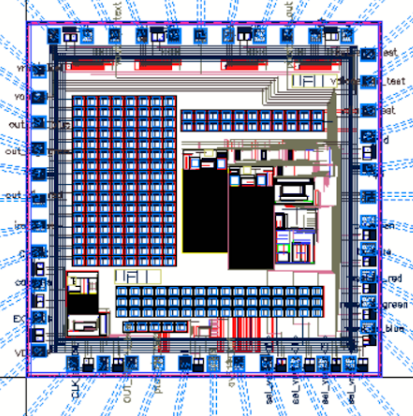
\includegraphics[scale=0.5]{Projeto/Layout/Imagens/CircuitoIntegrado.png}
    \legend{Fonte: Produzido pelo autor}
    \label{fig_circintegrado}
\end{figure}

\begin{figure}[!h]
 \centering
    \caption{Circuito Integrado utilizado para o Receptor Óptico particionado} 
    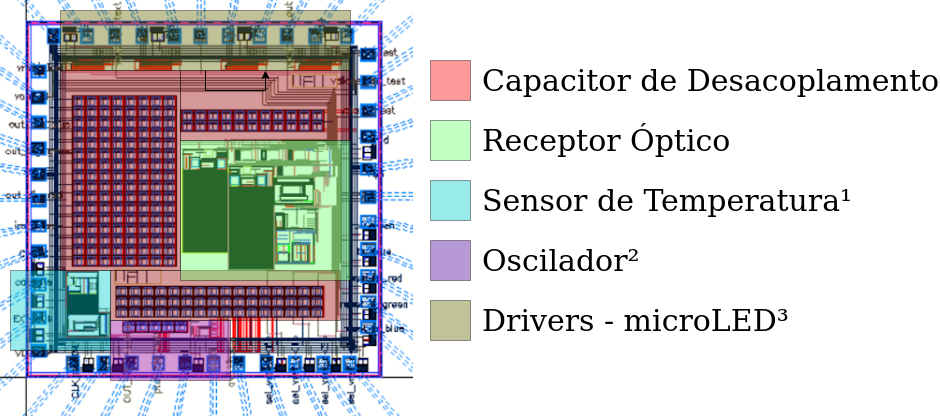
\includegraphics[scale=0.4]{Projeto/Layout/Imagens/Image_CircuitoIntegrado.png}
    \legend{Fonte: Roteamento de top-level realizados por Prof. Hugo, Daniel Lott e Prof. Dalton}
    \label{fig_circintegrado_division}
    \nota{\textsuperscript{1} Trabalho de Conclusão de Curso de Daniel Carvalho Lott \cite{DanielLott}\\\textsuperscript{2} Trabalho de Conclusão de Curso de Victor Rodrigues Barbosa \cite{VictorRodrigues}\\\textsuperscript{3} Trabalho realizado pelo aluno de Mestrado Rubens Alcântara de Souza, da UFMG}
\end{figure}

\begin{table}[!h]
\caption{Pinos presentes no circuito integrado para o Receptor Óptico}
\footnotesize
\begin{tabular}{cccll}
\toprule
\begin{tabular}[c]{@{}c@{}}Pino\\ Circuito \\ Integrado\end{tabular} & \begin{tabular}[c]{@{}c@{}}Pino\\ Chip\end{tabular} & Nome              & \multicolumn{1}{c}{Descrição}                                                                           & \multicolumn{1}{c}{Observação}                                                                                           \\
\midrule \midrule
1                                                                 & 40                                                  & vref\_pixel       & Não utilizado                                                                    &                                \\\midrule
2                                                                 & 41                                                  & vout\_clk         & Tensão de saída de relógio gerada                                                                       &                                \\\midrule
3                                                                 & 42                                                  & out\_dig\_blue    & \begin{tabular}[c]{@{}l@{}}Sinal de tensão digital\\ para cor azul\end{tabular}                         &                                \\\midrule
4                                                                 & 43                                                  & out\_dig\_green   & \begin{tabular}[c]{@{}l@{}}Sinal de tensão digital\\ para cor verde\end{tabular}                        &                                \\\midrule
5                                                                 & 44                                                  & VSS               & Terra                                                                                                   &                                \\\midrule
6                                                                 & 1                                                   & out\_dig\_red     & \begin{tabular}[c]{@{}l@{}}Sinal de tensão digital\\ para cor vermelha\end{tabular}                     &                                \\\midrule
7                                                                 & 2                                                   & iref\_test        & Não utilizado                                                                        &                                \\\midrule
23                                                                & 18                                                  & reset\_b\_blue    & \begin{tabular}[c]{@{}l@{}}Sinal de tensão de RESET\\ no APS para cor azul\end{tabular}                 & Ativo em nível baixo           \\\midrule
24                                                                & 19                                                  & reset\_b\_green   & \begin{tabular}[c]{@{}l@{}}Sinal de tensão de RESET\\ no APS para cor verde\end{tabular}                & Ativo em nível baixo           \\\midrule
25                                                                & 20                                                  & reset\_b\_red     & \begin{tabular}[c]{@{}l@{}}Sinal de tensão de RESET\\ no APS para cor vermelha\end{tabular}             & Ativo em nível baixo           \\\midrule
26                                                                & 21                                                  & tx\_blue          & \begin{tabular}[c]{@{}l@{}}Sinal de tensão de ENABLE\\ no APS para cor azul\end{tabular}                & Ativo em nível alto            \\\midrule
27                                                                & 22                                                  & tx\_green         & \begin{tabular}[c]{@{}l@{}}Sinal de tensão de ENABLE\\ no APS para cor verde\end{tabular}               & Ativo em nível alto            \\\midrule
28                                                                & 23                                                  & V18               & Tensão de alimentação de 1,8V                                                                           &                                \\\midrule
29                                                                & 24                                                  & VSS               & Terra                                                                                                   &                                \\\midrule
30                                                                & 25                                                  & tx\_red           & \begin{tabular}[c]{@{}l@{}}Sinal de tensão de ENABLE\\ no APS para cor vermelha\end{tabular}            & Ativo em nível alto            \\\midrule
31                                                                & 26                                                  & vdiode\_test      & \begin{tabular}[c]{@{}l@{}}Corrente que simula fotogeração\\ no APS de teste\end{tabular} &                                \\\midrule
32                                                                & 27                                                  & vdiode\_clk\_test & \begin{tabular}[c]{@{}l@{}}Corrente que simula fotogeração\\ no fotodiodo no TIA de teste\end{tabular} &                                \\\midrule
33                                                                & 28                                                  & out\_ana\_test    & \begin{tabular}[c]{@{}l@{}}Sinal de tensão analógico para o\\ APS de teste\end{tabular}                 &         \\\bottomrule                      
\end{tabular}
\label{tab_clcc44}
\legend{Fonte: Produzido pelo autor}
\end{table}